As a programmers, I believe all we have faced the cases of crucial over-engineering during the implementation of some
software product.
For the programmer, it is a vital point to follow two separated, but closely related software development principles,
such that KISS [INSERTREF], and YAGNI [INSERTREF].
As the main topic of our thesis is to implement Instant Messaging System following the security and privacy aspects.
We consider to following above-mentioned development principles KISS and YAGNI and approach
a well-known N-tier application Monolithic architecture [INSERTREF], which provides a model by which developers can
create flexible and reusable applications.
By segregating an application into tiers, developers acquire the option of modifying or adding a specific layer,
instead of reworking the entire application.
A three-tier architecture is typically composed of a presentation tier, a logic tier, and a data tier.
One would suggest to use nowadays popular Microservices Architecture, thinking about scalability [INSERTREF],
an ability of the system to handle large numbers of users distributed over geographically large areas without
notably affecting the overall performance of the system.
However, the effect of Microservices is being felt only for quite large and complex systems,
not the case of our yet simple application.
Following plot demonstrates this relation

\begin{figure}[H]
    \centering
    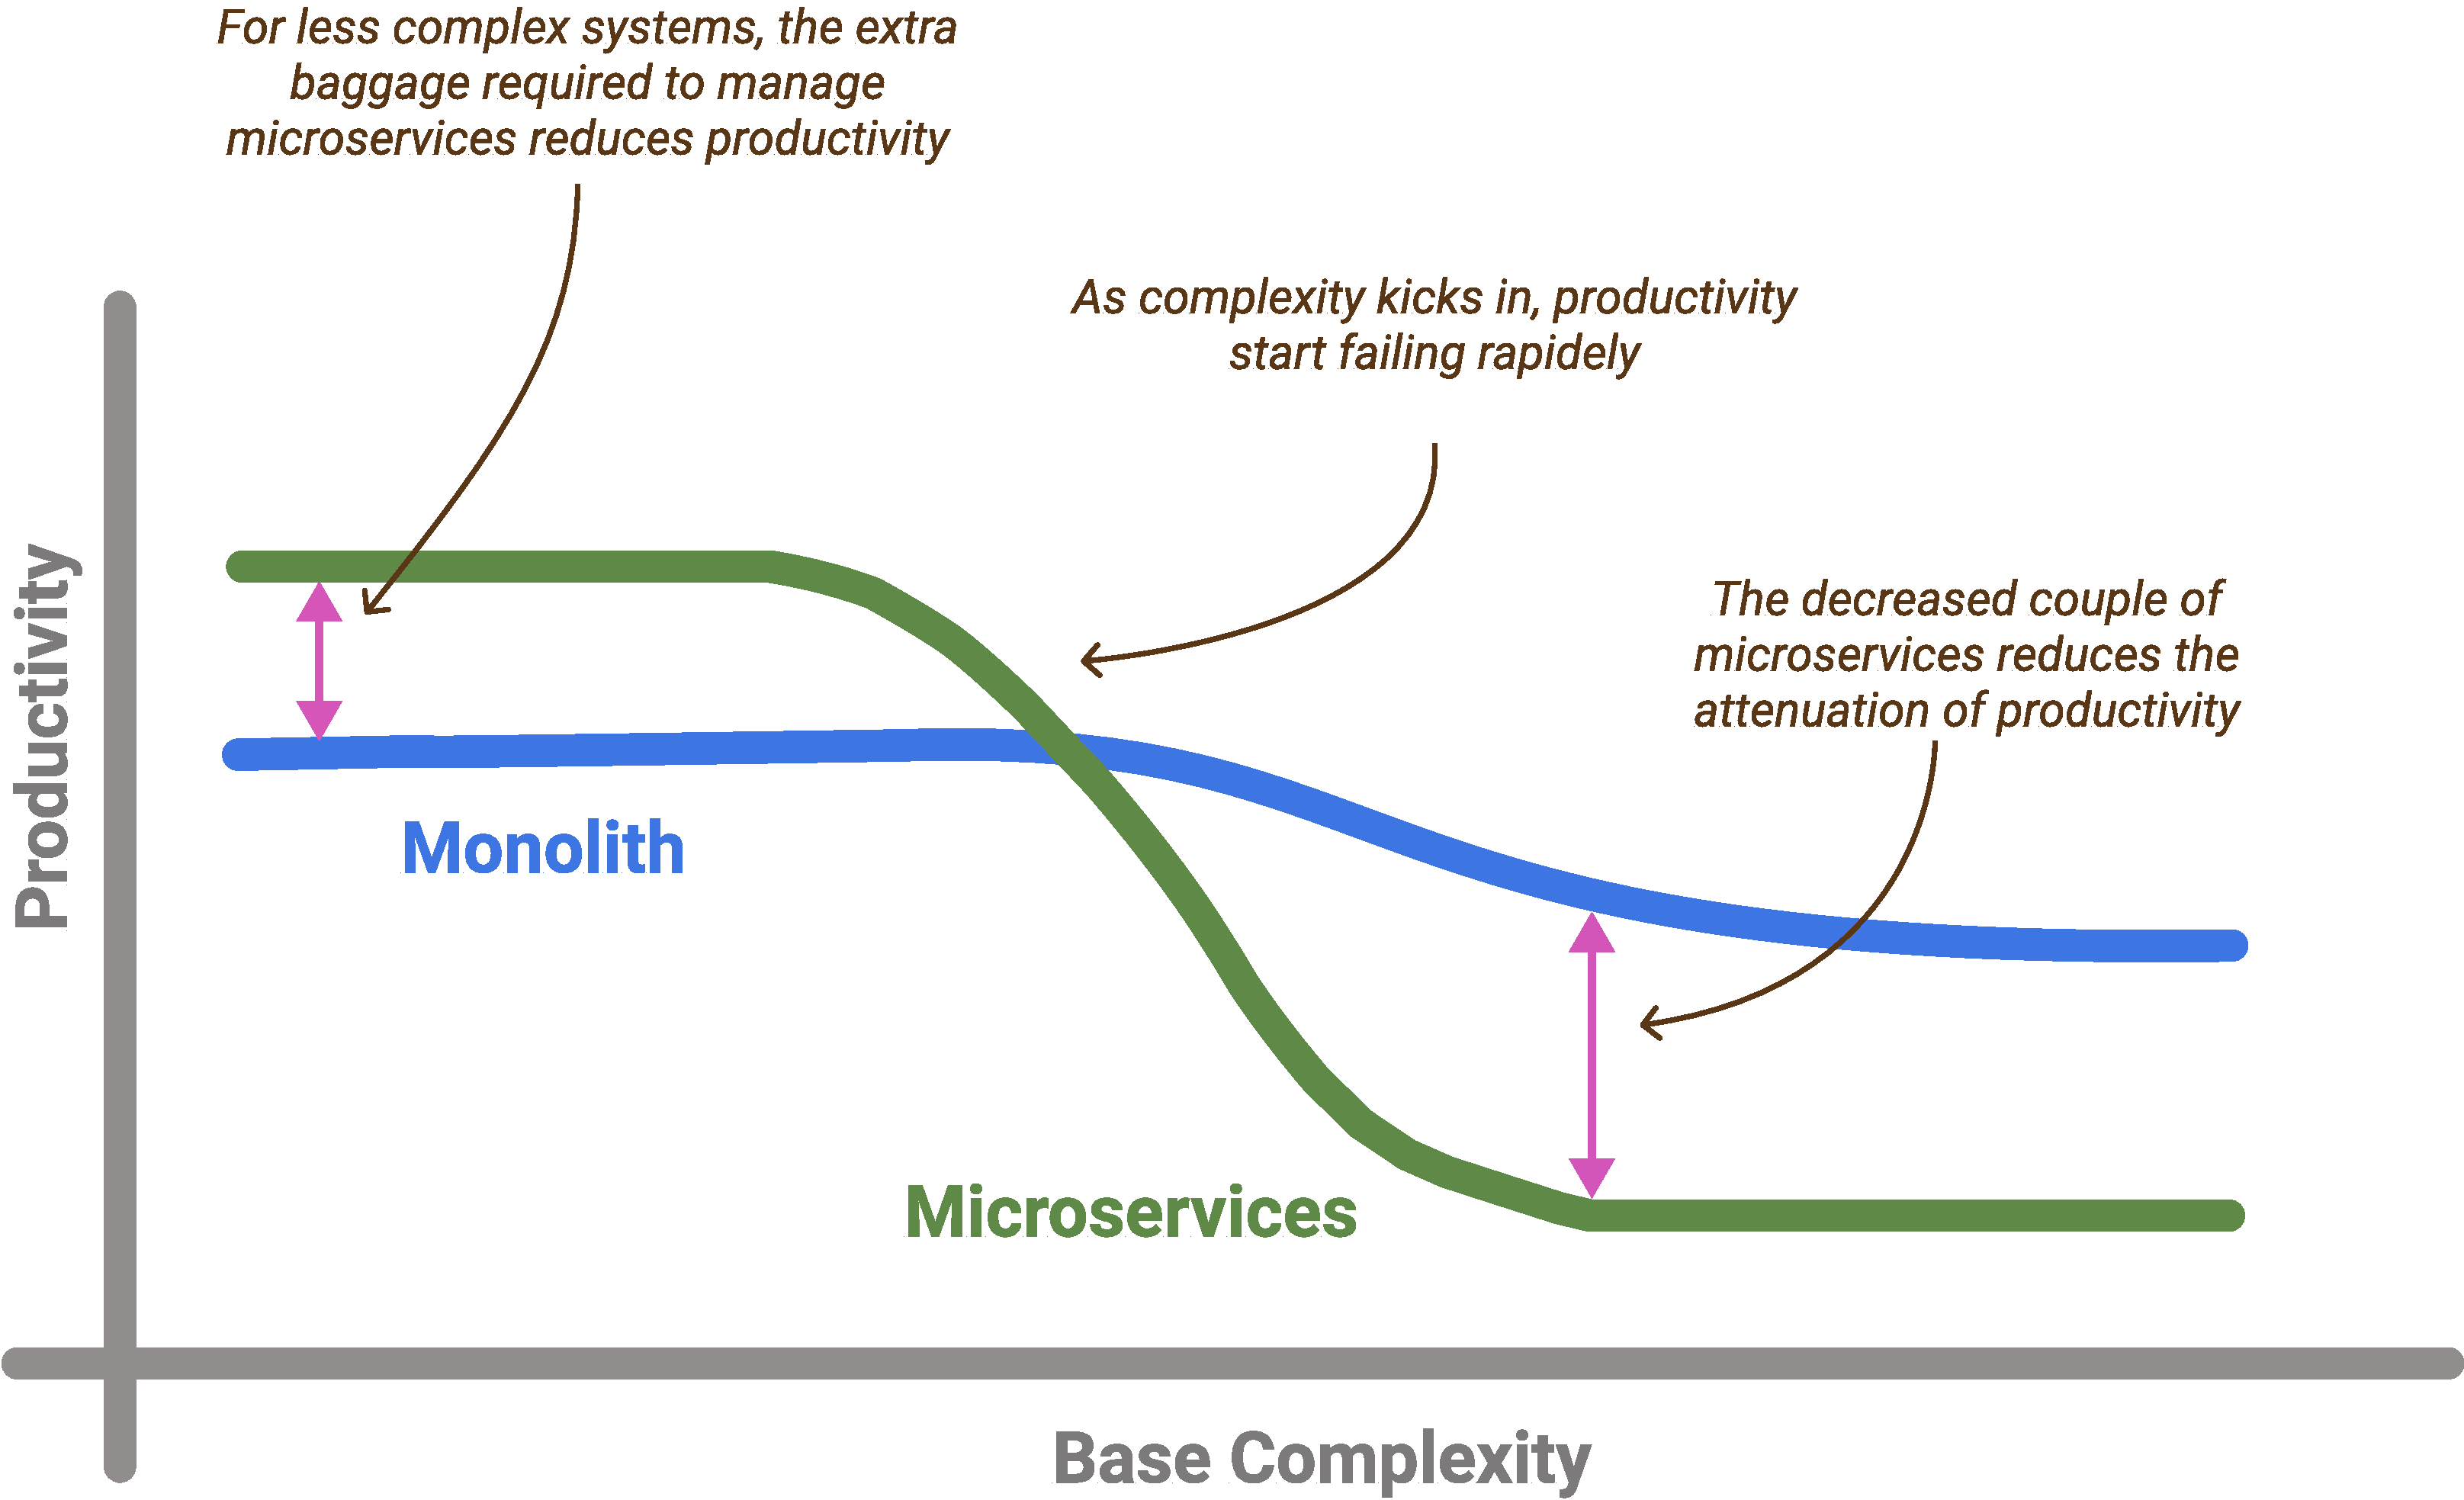
\includegraphics[width=1\textwidth]{Pictures/Monolith_vs_Microservice.pdf}
    \caption{Relation between system complexity and architectures. Source: https://martinfowler.com/bliki/MicroservicePremium.html}
    \label{fig:monolith_vs_microservice}
\end{figure}

In a logical multilayer architecture for an information system with an object-oriented design, the following four are the most common:

\begin{itemize} % source: https://en.wikipedia.org/wiki/Multitier_architecture#cite_note-5
    \item \textbf{Presentation Layer.} UI layer, view layer, presentation tier in multitier architecture.
    \item \textbf{Application Logic.} Service layer[5][6] or GRASP Controller Layer [7].
    \item \textbf{Business Logic.} Business logic layer (BLL), domain logic layer.
    \item \textbf{Data Access Layer.} Persistence layer, logging, networking, and other services which are required to support a particular business layer.
\end{itemize}

\begin{figure}[H]
    \centering
    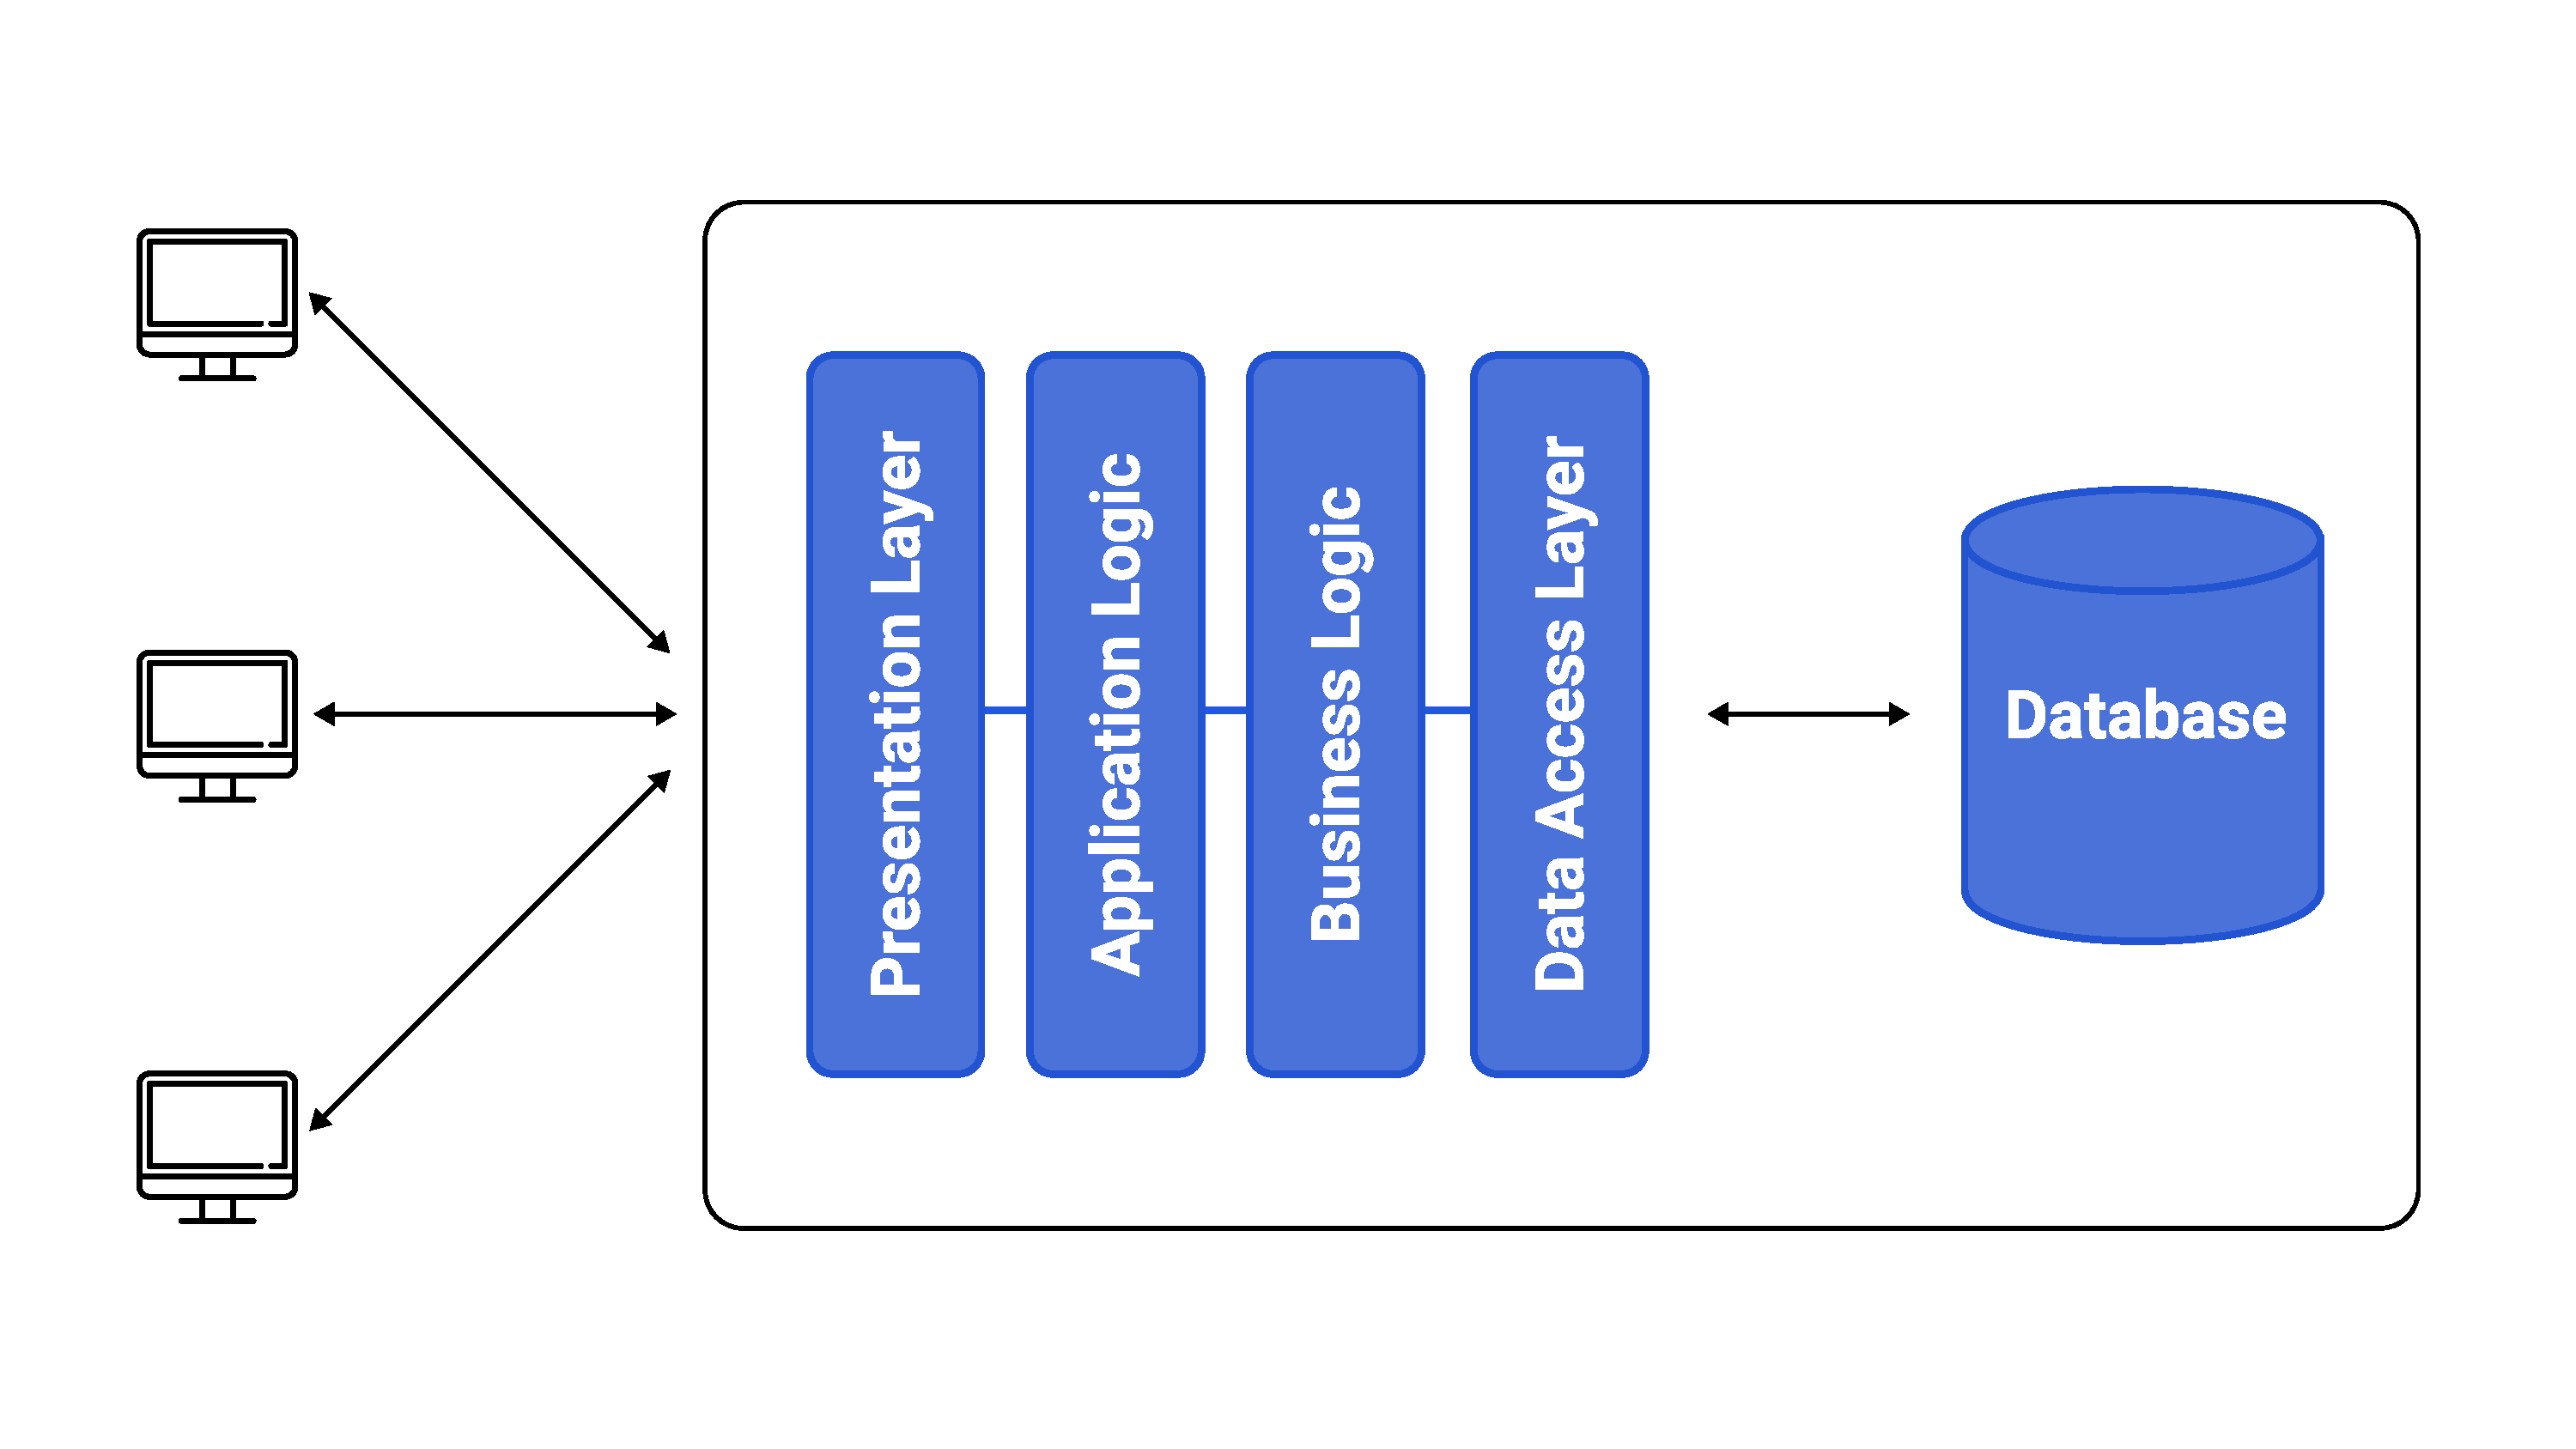
\includegraphics[width=1\textwidth]{Pictures/Monolith_architecture.pdf}
    \caption{Monolithic architecture diagram. Source: }\label{fig:figure2}
\end{figure}

The book Domain Driven Design describes some common uses for the above four layers, although its primary focus is the
domain layer.[8]
If the application architecture has no explicit distinction between the business layer and the presentation layer
(i.e., the presentation layer is considered part of the business layer), then a traditional client-server (two-tier)
model has been implemented.[citation needed]
The more usual convention is that the application layer (or service layer) is considered a sublayer of the business layer,
typically encapsulating the API definition surfacing the supported business functionality.
The application/business layers can, in fact, be further subdivided to emphasize additional sublayers of distinct
responsibility.
For example, if the model–view–presenter pattern is used, the presenter sublayer might be used as an additional layer
between the user interface layer and the business/application layer (as represented by the model sublayer).
Some also identify a separate layer called the business infrastructure layer (BI), located between the business layer(s)
and the infrastructure layer(s).
It's also sometimes called the "low-level business layer" or the "business services layer".
This layer is very general and can be used in several application tiers (e.g. a CurrencyConverter).[9]
The infrastructure layer can be partitioned into different levels (high-level or low-level technical services).[9]
Developers often focus on the persistence (data access) capabilities of the infrastructure layer and therefore only
talk about the persistence layer or the data access layer (instead of an infrastructure layer or technical services layer).
In other words, the other kind of technical services are not always explicitly thought of as part of any particular
layer.
A layer is on top of another, because it depends on it.
Every layer can exist without the layers above it, and requires the layers below it to function.
Another common view is that layers do not always strictly depend on only the adjacent layer below.
For example, in a relaxed layered system (as opposed to a strict layered system) a layer can also depend on all the layers below it.[4]

\subsection{Monolith Architecture: Cons and Props}\label{subsec:monolith-architecture:-cons-and-props}

A monolith is built as a large system with a single code base and deployed as a single unit, usually behind a load balancer.
It typically consists of four major components: a user interface, business logic, a data interface and a database.
Monoliths offer several advantages, particularly when it comes to operational overhead requirements.
Here are some of those basic benefits:

\begin{itemize}
    \item \textbf{Simplicity.} Monolithic architectures are simple to build, test and deploy.
    These apps can scale horizontally, in one direction, by running several copies of the application behind a load balancer.
    Cross-cutting concerns: With a single codebase, monolithic apps can easily handle cross-cutting concerns, such as logging,
    configuration management and performance monitoring.
    Another advantage associated with the simplicity of monolithic apps is easier deployment.
    When it comes to monolithic applications, you do not have to handle many deployments – just one file or directory.
    \item \textbf{Performance.} Components in a monolith typically share memory which is faster than service-to-service communications using
    IPC [INSERTREF] or other mechanisms.
    \item \textbf{Easier debugging and testing.}
    In contrast to the microservices architecture, monolithic applications are much easier to debug and test.
    Since a monolithic app is a single indivisible unit, you can run end-to-end testing much faster.
    \item \textbf{Easier development.} As long as the monolithic approach is a standard way of building applications,
    any engineering team has the right knowledge and capabilities to develop a monolithic application.
\end{itemize}
But one major drawback of monolithic architectures is tight coupling.
Over time, monolithic components become tightly coupled and entangled.
This coupling effects management, scalability and continuous deployment.
Other cons that stem from tight coupling include:

\begin{itemize}
    \item \textbf{Understanding.} When a monolithic application scales up, it becomes too complicated to understand.
    Also, a complex system of code within one application is hard to manage.
    \item \textbf{Reliability.} An error in any of the modules in the application can bring the entire application down.
    \item \textbf{Updates.} Due to a single large codebase and tight coupling, the entire application would have to deploy
    for each update.
    \item \textbf{Technology stack.} A monolithic application must use the same technology stack throughout.
    Changes to the technology stack are expensive, both in terms of the time and cost involved.
    \item \textbf{Scalability.} You cannot scale components independently, only the whole application.
\end{itemize}

\subsection{Decoupling Monolith using CQRS}\label{subsec:decoupling-monolith-using-cqrs}
As it stated in previous section, monolithic architecture provides a quite strong coupling between application
components.
Moreover, as monolith grow horizontally, its services layer grows as well.
This process leads to very huge code base which is very difficult to support and extend.
We attach the following
\href{https://github.com/smartstore/SmartStoreNET/blob/4.x/src/Presentation/SmartStore.Web/Controllers/CatalogHelper.cs}
{link}
as an example of such approach.
To avoid the natural results of monolithic architecture, that are huge classes for thousands lines, we have to dive into design patterns.
Precisely, the mediator pattern would help to decouple the service layer from presentation layer.
Mediator -- is a behavioral design pattern that lets you reduce chaotic dependencies between objects.
The pattern restricts direct communications between the objects and forces them to collaborate only via a mediator object.
In other words, mediator allows the communication between two entities, such that entities doesn't know each other.
The Mediator pattern suggests that you should cease all direct communication between the components which you want to make
independent of each other.
Instead, these components must collaborate indirectly, by calling a special mediator object that redirects the calls to
appropriate components.
As a result, the components depend only on a single mediator class instead of being coupled to dozens of their colleagues.

In context of .NET platform there are multiple implementation of the Mediator, the most widely known and used is the
\href{https://github.com/jbogard/MediatR}{MediatR}, which we use in our project.

Another, yet popular approach is the CQRS, which stands for Command-Query Responsibility Segregation.
In brief, it stands that read (query) and write (command) requests should be segregated by their responsibilities.
The CQRS approach in couple with Mediator greatly helps to solve the coupling problem of the monolith architecture.
So what is CQRS precisely?
According to Martin Fowler [INSERTREF],
It's a pattern that first described by Greg Young [INSERTREF].
At its heart is the notion that you can use a different model to update information than the model you use to read information.
For some situations, this separation can be valuable, but beware that for most systems CQRS adds risky complexity.
The mainstream approach people use for interacting with an information system is to treat it as a CRUD datastore.
By this meant that we have mental model of some record structure where we can create new records, read records,
update existing records, and delete records when we're done with them.
In the simplest case, our interactions are all about storing and retrieving these records.
As our needs become more sophisticated we steadily move away from that model.
We may want to look at the information in a different way to the record store, perhaps collapsing multiple records into one,
or forming virtual records by combining information for different places.
On the update side we may find validation rules that only allow certain combinations of data to be stored, or may even infer
data to be stored that's different from that we provide.
For instance, the idea of command-query segregation is displayed at the following image

\begin{figure}[H]
    \centering
    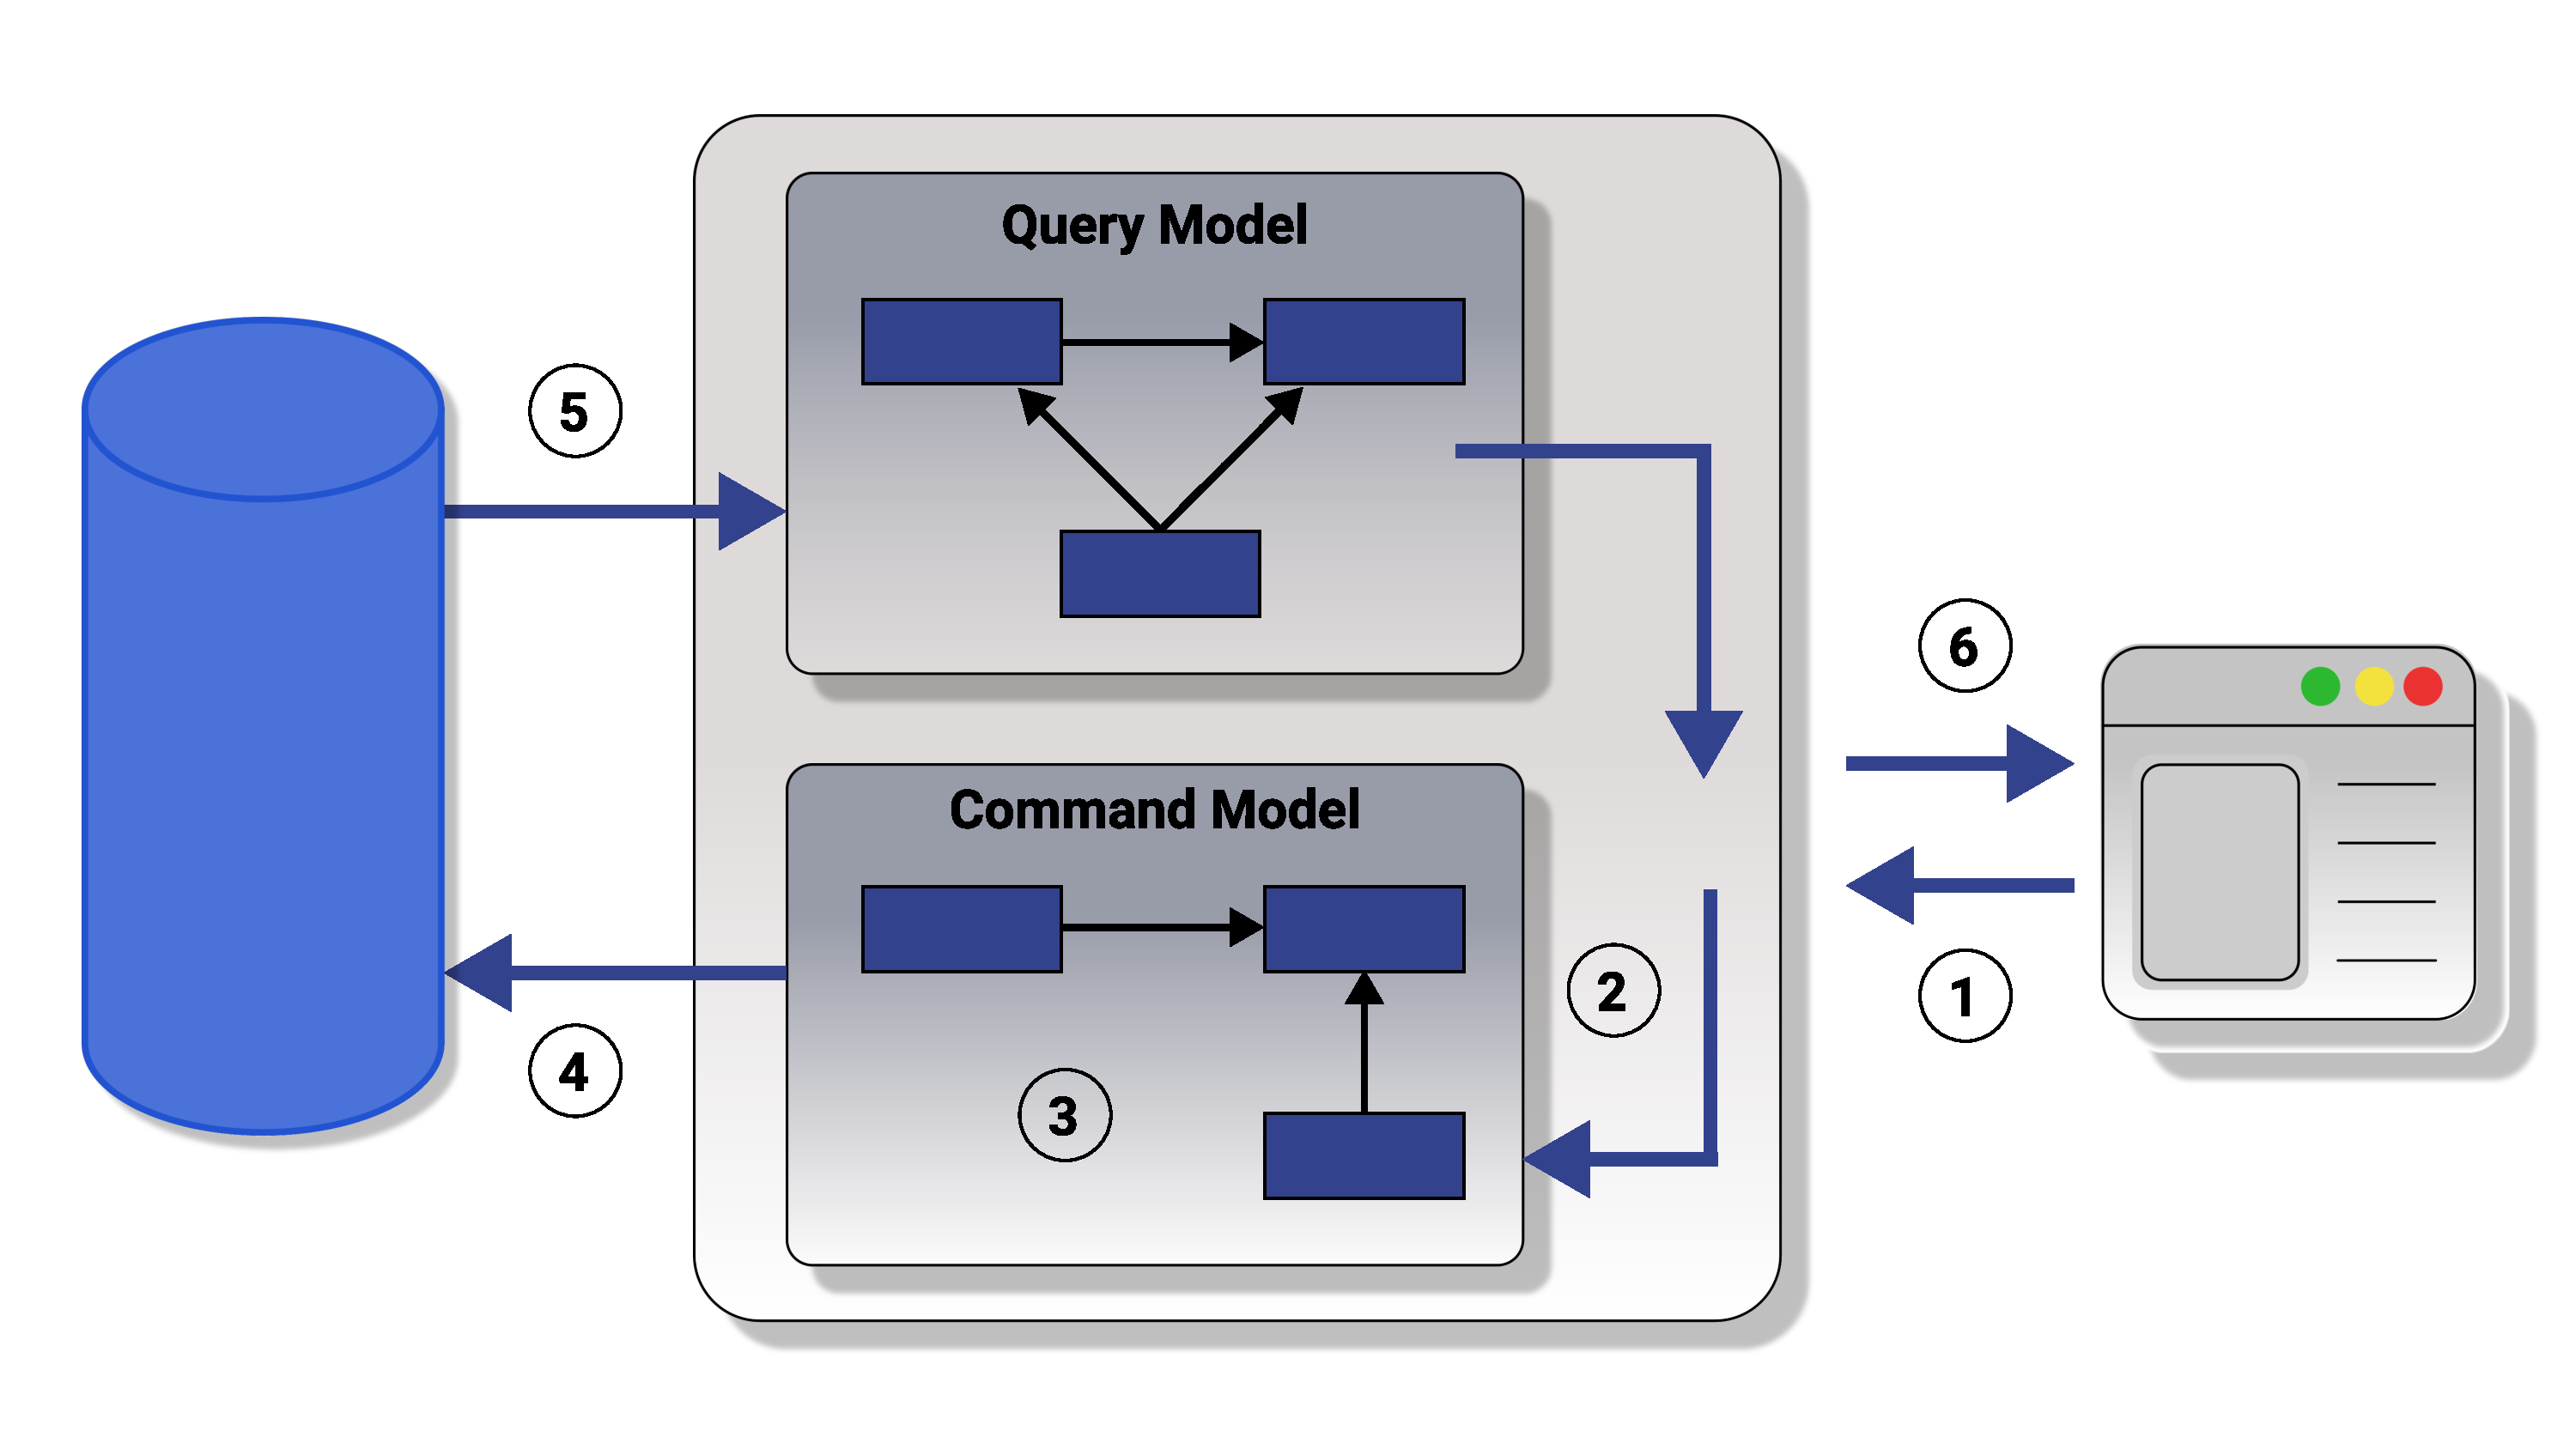
\includegraphics[width=1\textwidth]{Pictures/cqrs.pdf}
    \caption{CQRS Conceptual diagram. Source: https://martinfowler.com/bliki/CQRS.html}\label{fig:figure}
\end{figure}

Despite these benefits, you should be very cautious about using CQRS.
Many information systems fit well with the notion of an information base that is updated in the same way that it's read,
adding CQRS to such a system can add significant complexity.
I've certainly seen cases where it's made a significant drag on productivity, adding an unwarranted amount of risk to the
project, even in the hands of a capable team.
So while CQRS is a pattern that's good to have in the toolbox, beware that it is difficult to use well and you can easily
chop off important bits if you mishandle it.

As a short conclusion, we may state that CQRS and Mediator pattern will not entirely solve the coupling problems the monolith,
however will make project much more simplistic and intuitively understood.
It is worth to keep is simple,
even relatively simple project may grow to the sizes of universe without proper architectural solutions.

\subsection{Database Structure and related comments}\label{subsec:database-structure-and-related-comments}
As a next topic to uncover goes the one related to the database structure.
Proper database structure is to be of very high priority, since it influences on the project as a whole,
starting from performance point of view and many other aspects.
When we say performance, we mean such a design of database that there is an opportunity to include required indexes,
depending on regularity of any particular request.
So, as the main topic of current thesis is implementation of Instant messaging system, we can list the following
general entities to be added to database schema.

\begin{itemize}
    \item \textbf{Users.} Table stores information about user.
    Table contains following columns:
    \begin{itemize}
        \item Id VARCHAR(36) -- Id of the user, primary key, Guid.
        \item UserName VARCHAR(50) -- Unique Username.
        \item NormalizedUserName VARCHAR(50) -- Unique Username in upper case.
        \item DisplayName VARCHAR(50) -- Name of the user, displayed to others.
        \item Bio VARCHAR(250) -- User's short biography, visible to others.
        \item Image VARCHAR(36) -- User's profile picture, visible to others.
        \item Email VARCHAR(120) -- User's email address, not public.
        \item EmailConfirmed BOOLEAN -- Flag that indicates if user has confirmed his email address.
        \item PhoneNumber VARCHAR(50) -- User's phone number.
        \item PhoneNumberConfirmed BOOLEAN -- Flag that indicates if user has confirmed his phone number.
        \item PhoneVerificationCode INTEGER -- Code sent to user in order to confirm phone number.
        \item PasswordHash VARCHAR(60) -- Hashed password.
        \item CreatedAt DATETIME -- Indicates the date and time user has been registered.
        \item UpdatedAt DATETIME -- Indicates the date and time user has updated his record.
    \end{itemize}
    \item \textbf{User Personal Information.} Table stores additional but not required info about user.
    Relation one-to-one with Users, foreign key is UserId, Guid.
    Table contains following columns:
    \begin{itemize}
        \item UserId VARCHAR(36) -- Foreign key to the Users table, Guid.
        \item FirstName VARCHAR(120) -- First name of user.
        \item LastName VARCHAR(120) -- Last name of user.
        \item BirthDay DATETIME -- Birth day of user.
        \item WebSite VARCHAR(120) -- Web site of user.
        \item Address VARCHAR(120) -- Residence address of user.
        \item Facebook VARCHAR(120) -- Facebook nickname of user.
        \item Twitter VARCHAR(120) -- Twitter nickname of user.
        \item Instagram VARCHAR(120) -- Instagram nickname of user.
        \item LinkedIn VARCHAR(120) -- LinkedIn nickname of user.
        \item ProfilePicture VARCHAR(36) -- Avatar of user.
    \end{itemize}
    \item \textbf{UserContacts.} Table stores the contacts of current user.
    Relation between tables Users and UserContacts is one-to-many, foreign key UserId.
    Table contains following columns:
    \begin{itemize}
        \item ContactId VARCHAR(36) -- Id of current user's contact, Guid.
        \item UserId VARCHAR(36) -- Id of current user, Guid.
    \end{itemize}
    \item \textbf{Chats.} In order to communicate with other people it is essentially to have a chat room.
    Our implementation provides chat rooms of the four types.
    Direct chat -- chat room between only two members.
    Public channel -- chat room for multiple members, each member can send and read messages.\ It displayed in search results.
    Readonly channel -- channel for multiple members, however only the owner can send messages.\ It displayed in search results.
    Private channel -- channel for multiple members, can be joined only by invite link.
    Each user can have a numerous various chats, however, each chat has a multiple members, at least 2 as the case of direct chat.
    Therefore, we consider a many-to-many relation between user and chats via intermediate table UserChats.
    We discuss UserChats relation in foregoing part.
    Continuing with Chats table, it contains the following columns:
    \begin{itemize}
        \item Id VARCHAR(36) -- Id of the chat, primary key, Guid.
        \item ChatInfoId VARCHAR(36) -- Since we have a four types of channels, which has a common subset of data,
        the different data is moved to another table, so it could be joined depending on chat type.
        For instance, any chat type except direct one would require to join additional data in order to display the chat properly.
        \item Title VARCHAR(50) -- Simply, the title of the chat.
        \item Image VARCHAR(36) -- Picture of the chat.\ Displayed in search results etc.
        \item ChatType ENUM -- The type of the chat, e.g direct chat, public channel, readonly channel, private channel.
        \item CreatedAt DATETIME -- Indicates the date and time chat has been created.
        \item UpdatedAt DATETIME -- Indicates the date and time chat has been updated.
    \end{itemize}
    \item \textbf{UserChats.} Table that considered as composite key of the many-to-many relation between Users and Chats tables.
    Over that, contains an enum value that indicates user's role in the chat.
    We assume the following user roles in the system:
    \begin{itemize}
        \item Owner -- the creator of the chat.
        Has an ultimate privileges.
        \item Administrator -- designated by the owner user, which has adjustable privileges.
        \item Moderator -- designated by administrator user, which has adjustable privileges.
        \item User -- default role assigned to the user on join the chat.
    \end{itemize}
    Despite that, the UserChats table contains the following columns:
    \begin{itemize}
        \item ChatId VARCHAR(36) -- Foreign key to the Chats table, Guid.
        \item UserId VARCHAR(36) -- Foreign key to the Users table, Guid.
        \item RoleId ENUM -- Indicates the user role in the chat, e.g Owner, Administrator, Moderator, User.
    \end{itemize}
    \item \textbf{Chat Info.} Table contains additional data related to the chat.
    This table is created since that we have four types of chats, namely, direct chat, public channel,
    readonly channel, private channel.
    These four types has a common data between each other.
    Common data between chat types is Chats table itself.
    One would advise to store the chats in a single table per chat type, however it is very costly approach, since there
    would be at least four joins per request.
    Note that every chat type except direct chat requires an additional data to be displayed, that is Chat Info.
    Contains following columns:
    \begin{itemize}
        \item Id VARCHAR(36) -- Id of the chat information, primary key, Guid.
        \item Description VARCHAR(120) -- Description of the chat.
        \item Tag VARCHAR(20) -- Uniqu identifier of the chat.
        \item MembersCount INTEGER -- Count of members in the chat.
    \end{itemize}
    \item \textbf{Messages.} Table that keeps messages and related data.
    Each chat has a multiple messages, however one message must belong only to single and defined chat,
    therefore relation between Chats and Messages is one-to-many, foreign key ChatId.
    From other side, each User has a multiple messages, however single message should belong to single author,
    therefore, we consider one-to-mane relation between Users and Messages, foreign key UserId.
    Messages table contains following columns:
    \begin{itemize}
        \item Id VARCHAR(36) -- Id of the message, primary key, Guid.
        \item ChatId VARCHAR(36) -- Foreign key to the Chats table, Guid.
        \item UserId VARCHAR(36) -- Foreign key to the Users table, Guid.
        \item Content VARCHAR(300) -- Content of the message.
        \item IsRead BOOLEAN -- Indicates whenever message has been read by another user.
        \item CreateAt DATETIME -- Time when the message has been created.
        \item UpdatedAt DATETIME -- Time when the message has been updated.
    \end{itemize}
    \item \textbf{Refresh Tokens.} Table stores refresh tokens.
    \begin{itemize}
        \item Id VARCHAR(36) -- Id of the token, primary key, Guid.
        \item UserId VARCHAR(39) -- Foreign key to the Users table, Guid.
        \item RefreshToken VARCHAR(60) -- Refresh token itself.
        \item Expires DATETIME -- Expiration date of refresh token.
        \item CreatedAt DATETIME -- Date when token has been created.
    \end{itemize}
\end{itemize}
Following diagram demonstrates the database structure.
\begin{figure}[H]
    \centering
    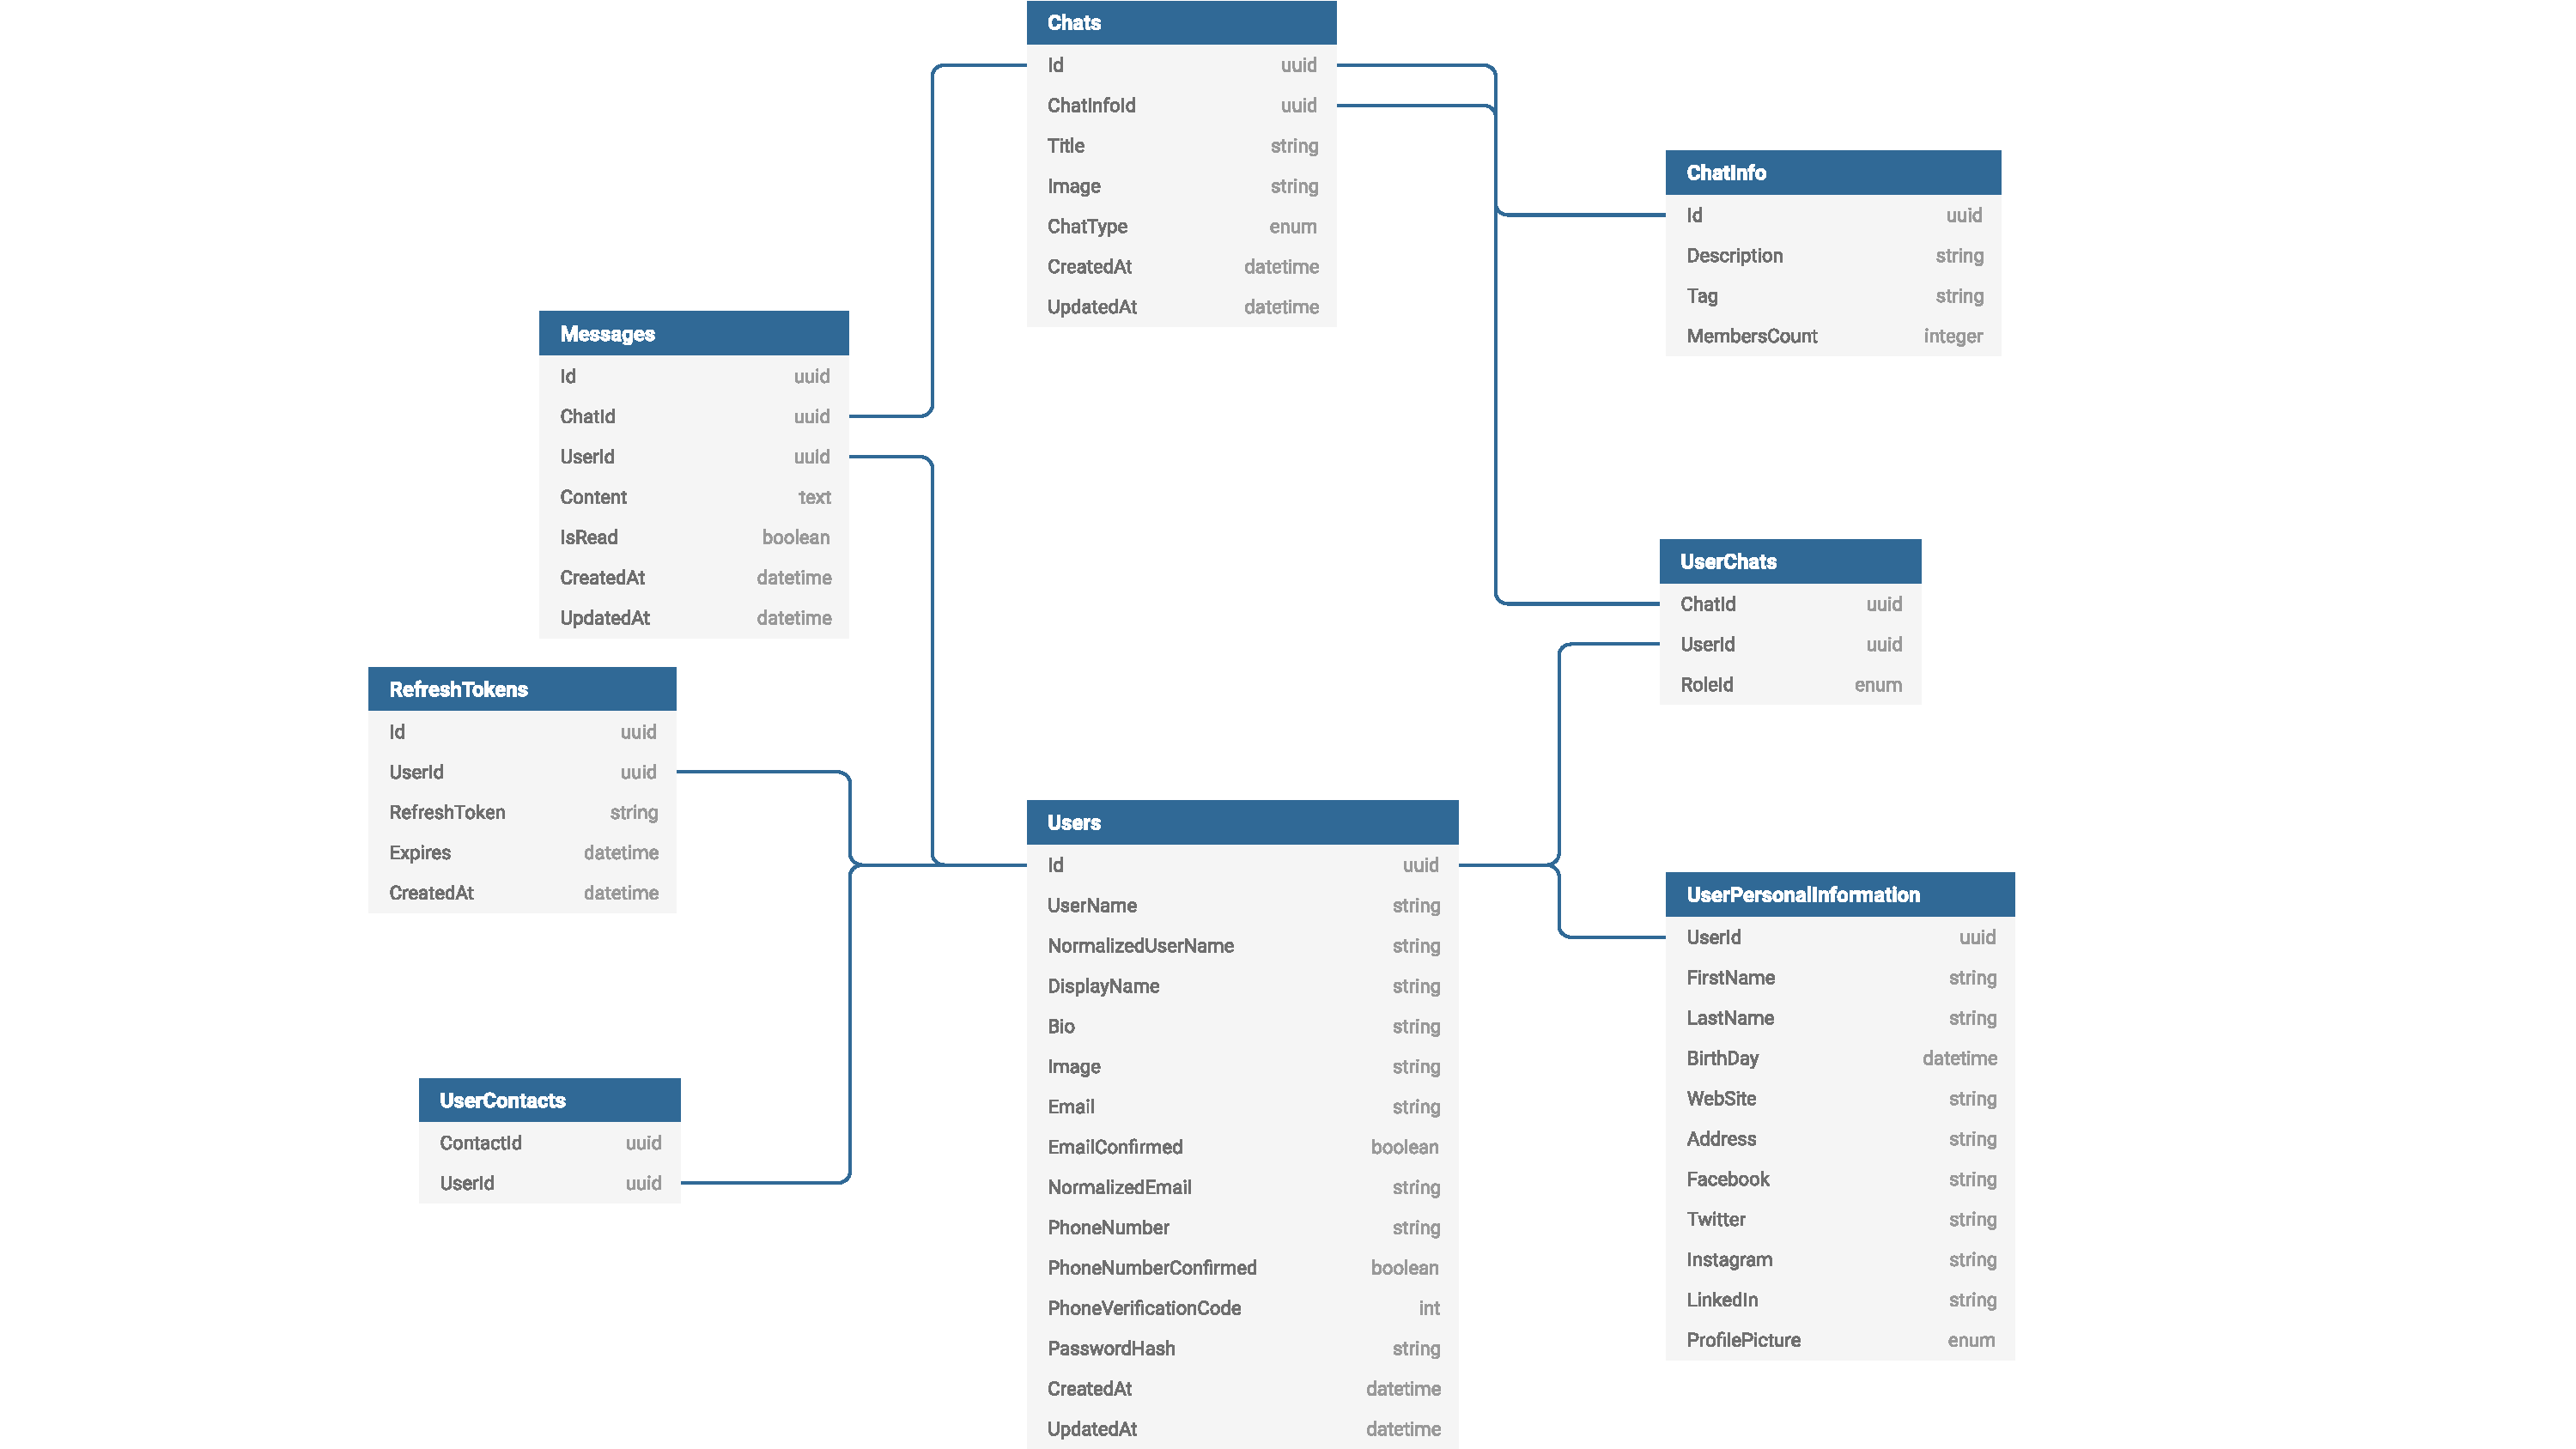
\includegraphics[width=1.2\textwidth]{Pictures/DB_diagram}
    \caption{Database diagram}\label{fig:figure5}
\end{figure}
Over whole data entities, we prefer to use universally unique identifier (UUID) or namely globally unique identifier (GUID),
a 128-bit label used for information in computer systems.
Simply, because it does not force us to keep a sequence on database side.
Sequence -- is a special entity provided in PostgreSQL relational databases.
It is responsible for generating unique values and sometimes causes a problems during migration of the databse.
But still, are GUID identifiers are really always unique?
Well, each generated GUID is not guaranteed to be unique, the total number of unique keys $2^{128}$ or $3.4 \times 10^{38}$
is so large that the probability of the same number being generated twice is very small.
For example, consider the observable universe, which contains about $5 \times 10^{22}$ stars.
Every star could then have $6.8 \times 10^{15}$ universally unique GUIDs.
If you are scared of the same GUID values then put two of them next to each other.
If you are too paranoid then put three [\cite{GuidSo}].

\subsection{Authentication and Authorization processes}\label{subsec:authentication-and-authorization-processes}
In this section we describe the processes of Authentication and Authorization in the system.
It is worth to remember the meaning of Authentication and Authorization definitions.
Authentication -- is the process of ascertaining that somebody really is who they claim to be.
Authorization refers to rules that determine who is allowed to do what.
For example, Adam may be authorized to create and delete databases, while Eve is only authorized to read.
The two concepts are completely orthogonal and independent, but both are central to security design, and the
failure to get either one correct opens up the avenue to compromise.
In terms of web apps, very crudely speaking, authentication is when you check login credentials to see if you recognize
a user as logged in, and authorization is when you look up in your access control whether you allow the user to view,
edit, delete or create content.
As to the projects concerns, we should handle multiple client applications, e.g desktop, web, mobile etc.
Therefore, cookie authorization doesn't fit for the project, however the JWT one surely passes.
So, what is JSON Web Token (JWT)?
JSON Web Token (JWT) is an open standard (RFC 7519) that defines a compact and self-contained way for securely
transmitting information between parties as a JSON object.
This information can be verified and trusted because it is digitally signed.
JWTs can be signed using a secret (with the HMAC algorithm) or a public/private key pair using RSA or ECDSA.
Although JWTs can be encrypted to also provide secrecy between parties, we will focus on signed tokens.
Signed tokens can verify the integrity of the claims contained within it, while encrypted tokens hide those claims from
other parties.
When tokens are signed using public/private key pairs, the signature also certifies that only the party holding the
private key is the one that signed it.
In its compact form, JSON Web Tokens consist of three parts separated by dots (.), which are:
\begin{itemize}
    \item Header -- typically consists of two parts: the type of the token, which is JWT, and the signing algorithm
    being used, such as HMAC SHA256 or RSA.
    \item Payload -- The second part of the token is the payload, which contains the claims.
    Claims are statements about an entity (typically, the user) and additional data.
    There are three types of claims: registered, public, and private claims.
    \item Signature -- To create the signature part you have to take the encoded header, the encoded payload, a secret,
    the algorithm specified in the header, and sign that.
\end{itemize}
Therefore, a JWT typically looks like \texttt{xxxxx.yyyyy.zzzzz}.
Then, this JSON is Base64Url encoded to form the first part of the JWT.
How do JSON Web Tokens work?
n authentication, when the user successfully logs in using their credentials, a JSON Web Token will be returned.
Since tokens are credentials, great care must be taken to prevent security issues.
In general, you should not keep tokens longer than required.
You also should not store sensitive session data in browser storage due to lack of security.
Whenever the user wants to access a protected route or resource, the user agent should send the JWT,
typically in the Authorization header using the Bearer schema.
The content of the header should look like \texttt{Authorization: Bearer <token>}.
This can be, in certain cases, a stateless authorization mechanism.
The server's protected routes will check for a valid JWT in the Authorization header, and if it's present, the user
will be allowed to access protected resources.
If the JWT contains the necessary data, the need to query the database for certain operations may be reduced, though
this may not always be the case.
If the token is sent in the Authorization header, Cross-Origin Resource Sharing (CORS) won't be an issue as it doesn't
use cookies.
The following diagram shows how a JWT is obtained and used to access APIs or resources:
\begin{figure}[H]
    \centering
    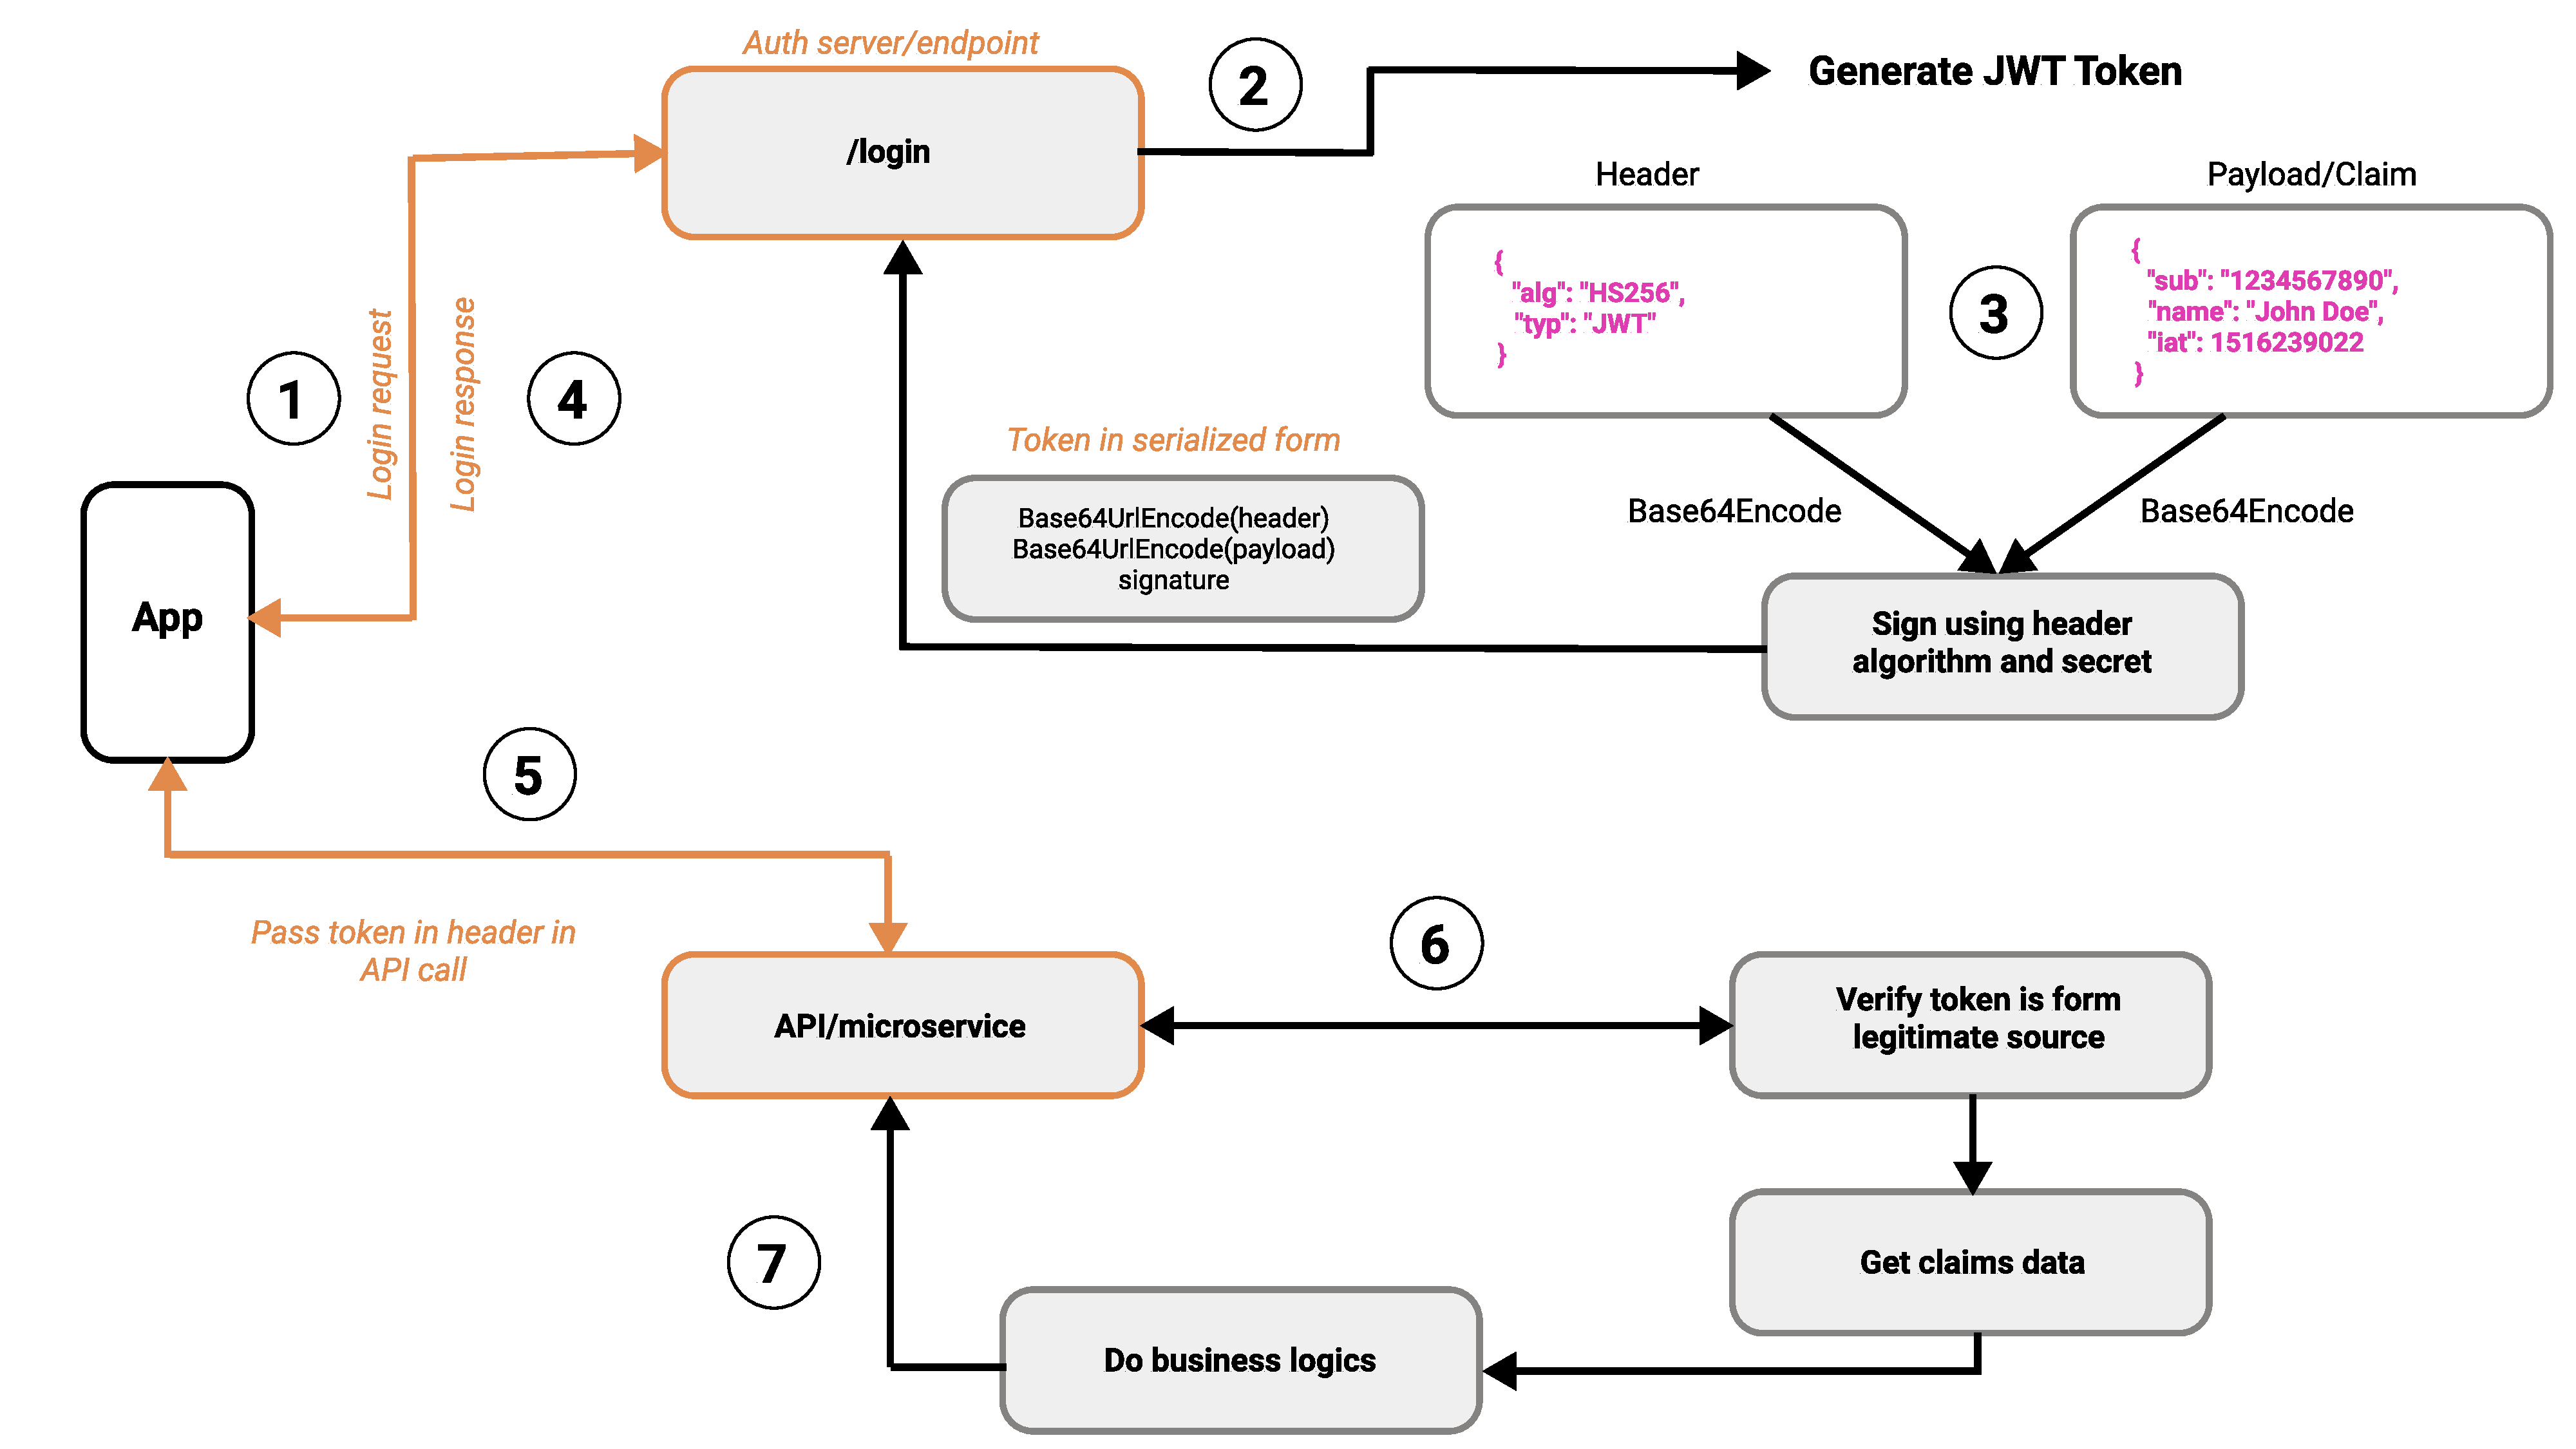
\includegraphics[width=1\textwidth]{Pictures/jwt_auth_scheme.pdf}
    \caption{JWT Authentication principle diagram.}\label{fig:figure3}
\end{figure}
JWT is quite simple and straightforward way to authorize particular person to the system's part.
However, what is about security, does it provide enough level of security?
Not really is.
When the JWT token is stolen, there is no way to revoke it.
Only the thing is to wait while token expires by himself, after its predefined lifetime.
A few basic rules about JWT usage [\cite{RDegges}]
\begin{itemize}
    \item JWT should have a short lifetime (few seconds).
    \item JWT should be used in a single time, e.g JWT per request.
\end{itemize}